% -*-coding: utf-8 -*-

\defaultfont

\BiChapter{基于单目视觉的目标定位与抓取策略研究}{To Template Maintainers}
\BiSection{引言}{Simple Introduction about This Template}

在水下作业环境中，机械臂仅依靠预设的轨迹无法快速完成动态变化的任务。本章设计
了一套基于单目视觉的定位系统，利用单目相机结合 OpenCV，通过内参
标定与 ArUco 手眼标定，构建了从图像像素坐标系到机械臂坐标系的空间映射关系。

\BiSection{单目相机成像模型}{Subsubsection}
针孔成像模型是视觉定位的几何基础，其描述了三维空间点与二维图像像素点之间的透射投影关系。该模型将世界坐标系中的点经刚体变换和相似三角形投影映射到成像平面，再由像素采样转换为离散坐标。整个过程可借助内参矩阵与外参矩阵，以齐次线性方程的形式紧凑表达。
%   \BiSubsection{坐标系定义与转换}{Subsubsection}

  为了描述目标位姿，本研究定义了四个关键坐标系，其转换逻辑如表 \ref{tab:coordinates} 所示。

  \begin{table}[htbp]
    \centering
    \caption{视觉系统坐标系定义}
    \label{tab:coordinates}
    \begin{tabular}{cccc}
        \toprule[2pt]   % 上粗线
        坐标系名称 & 符号 & 单位 & 物理意义 \\
        \midrule
        世界坐标系 & $\{W\}$ & m & 描述目标在环境或基座中的绝对位置 \\
        相机坐标系 & $\{C\}$ & mm & 以相机光心为原点，光轴为 $Z$ 轴 \\
        图像物理坐标系 & $\{p\}$ & mm & 投影点在感光元件上的连续物理位置 \\
        像素坐标系 & $\{uv\}$ & pixel & 图像在计算机存储中的离散像素索引 \\
        \bottomrule[2pt] % 下粗线
    \end{tabular}
\end{table}
% \BiSubsection{相机变换方程}{Subsubsection}
如图\ref{pic51}设空间目标点在相机坐标系下的坐标为 $\mathbf{P}_c = [X_c, Y_c, Z_c]^T$，其映射至像素坐标系下齐次坐标 $\mathbf{p} = [u, v, 1]^T$ 的变换过程可表示为：
\begin{equation}
    Z_c \begin{bmatrix} u \\ v \\ 1 \end{bmatrix} = \mathbf{K} \begin{bmatrix} X_c \\ Y_c \\ Z_c \end{bmatrix} = \begin{bmatrix} f_x & 0 & c_x \\ 0 & f_y & c_y \\ 0 & 0 & 1 \end{bmatrix} \begin{bmatrix} X_c \\ Y_c \\ Z_c \end{bmatrix}
\end{equation}
其中，$\mathbf{K}$ 为相机内参矩阵，$f_x, f_y$ 为等效像素焦距，$(c_x, c_y)$ 为主点坐标，$Z_c$ 为目标点在相机坐标系下的深度信息，即尺度因子。

\begin{figure}[H] % htbp代表图片插入位置的设置
    \centering %图片居中
    %添加图片；[]中为可选参数，可以设置图片的宽高；{}中为图片的相对位置
    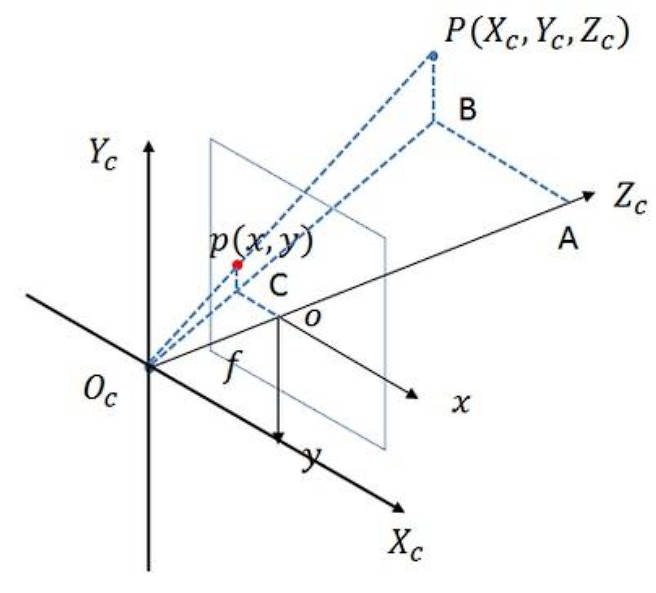
\includegraphics[width = 0.4\textwidth]{figures/xianji.jpg}
    \caption{相机变化示意图} % 图片标题
    \label{pic51} % 图片标签
    \vspace{-0.5cm}
    \end{figure}
  

此外，在水下等特殊介质或采用广角镜头时，图像会产生畸变。本系统引入如下多项
式畸变模型进行修正：
\begin{equation}
    \left\{
    \begin{aligned}
        x_{corrected} &= x(1 + k_1 r^2 + k_2 r^4 + k_3 r^6) + 2p_1 xy + p_2(r^2 + 2x^2) \\
        y_{corrected} &= y(1 + k_1 r^2 + k_2 r^4 + k_3 r^6) + p_1(r^2 + 2y^2) + 2p_2 xy
    \end{aligned}
    \right.
    \end{equation}

其中，$k_1, k_2, k_3$ 为径向畸变系数，$p_1, p_2$ 为切向畸变系数，$r^2 = x^2 + y^2$。

\BiSubsection{参数获取}{Subsubsection}

为了获取相机的内参矩阵 $\mathbf{K}$ 与畸变系数 $\mathbf{D}$，本研究采用了经
典的张正友
平面标定法。该方法仅需利用打
印的黑白棋盘格在不同位姿下的图像即可实现高精度标定。

张正友标定法的核心在于利用单应性矩阵描述棋盘格平面到图像平面的映射关系。
设定棋盘格所在
平面为 $Z_w = 0$，则空间点 $\mathbf{P}_w$ 与像素点 $\mathbf{p}$ 的关系简化为：
\begin{equation}s \mathbf{p} = \mathbf{K} \begin{bmatrix} \mathbf{r}_1 & \mathbf{r}_2 
    & \mathbf{t} \end{bmatrix} \begin{bmatrix} X_w \ Y_w \ 1 \end{bmatrix} 
    = \mathbf{H} \begin{bmatrix} X_w \ Y_w \ 1 \end{bmatrix}
\end{equation}
其中，$\mathbf{H}$ 为 $3 \times 3$ 的单应性矩阵。由于旋转矩阵的列向量 $\mathbf{r}_1$ 
和 $\mathbf{r}_2$ 有正交性，即满足：\begin{equation}\begin{cases}\mathbf{r}_1^T
     \mathbf{r}_2 = 0 \|\mathbf{r}_1| = |\mathbf{r}_2| = 1\end{cases}\end{equation}通
     过每张棋盘格图像提供的两个基本约束方程，在拍摄 3 张以上不同角度的照片后，即可线
     性解算出内参矩阵 $\mathbf{K}$。

     实验采用 ROS 2 环境下的标准标定工具包，通过实机采集数据并在线计算，获取相机的内参矩阵与畸变系数。


实验采用高平整度的黑白棋盘格作为标定板如图\ref{pic52}。
\begin{figure}[H] % htbp代表图片插入位置的设置
    \centering %图片居中
    %添加图片；[]中为可选参数，可以设置图片的宽高；{}中为图片的相对位置
    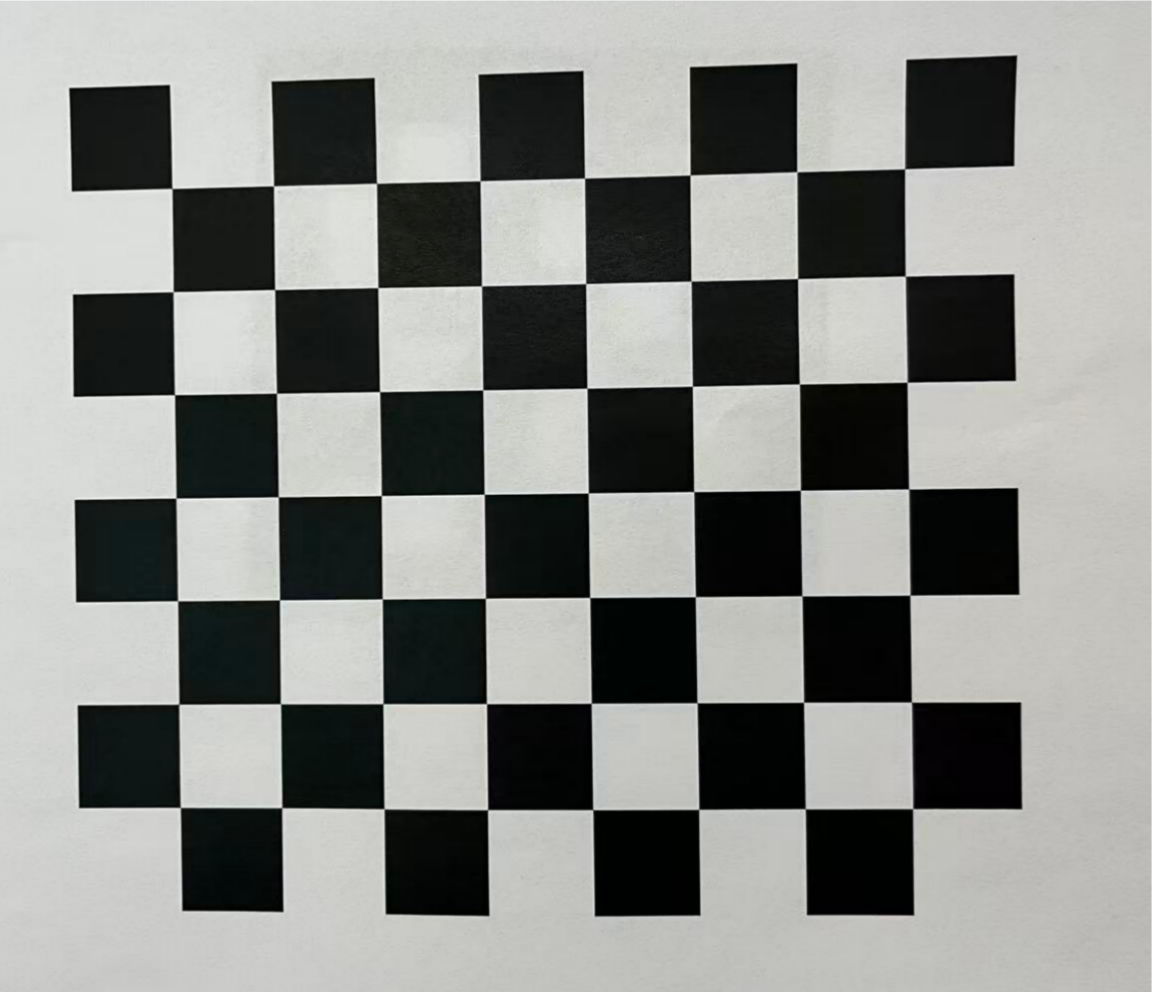
\includegraphics[width = 0.6\textwidth]{figures/5c90b1d64026c1610617104461e4ffd6.jpg}
    \caption{标定板} % 图片标题
    \label{pic52} % 图片标签
    \vspace{-0.5cm}
    \end{figure}
为了标定算法可以订阅到正确的图像流并解析其物理尺度，标定程序的启动参数配置如表 \ref{tab:ros_calib_params} 所示。

\begin{table}[htbp]
    \centering
    \caption{ROS 2 标定程序指令参数说明}
    \label{tab:ros_calib_params}
    \begin{tabular}{lp{3cm}l}
        \toprule[2pt]
        参数名称 & 实验设定值 & 功能描述 \\
        \midrule
        \texttt{size} & $7 \times 8$ & 棋盘格内部角点数量 \\
        \texttt{square} & $0.017$ & 单个方格物理边长 (m) \\
        \texttt{p} & \texttt{chessboard} & 指定标定板类型为棋盘格 \\
        \texttt{remap} & \texttt{/raw\_image} & 映射相机原始图像话题 \\
        \bottomrule[2pt]
    \end{tabular}
\end{table}



标定过程中，如图\ref{pic53}通过手动变换标定板相对于相机镜头的位姿，标定工具箱实时监测四个关键维度的样本覆盖率：

（1）X \& Y：反映标定板在图像视野水平与垂直方向上的偏移量。

（2）Size：反映标定板相对于相机的远近变化，用于校核尺度因子。

（3）Skew：反映标定板的倾斜角度，用于解算成像平面的旋转约束。


\begin{figure}[H] % htbp代表图片插入位置的设置
    \centering %图片居中
    %添加图片；[]中为可选参数，可以设置图片的宽高；{}中为图片的相对位置
    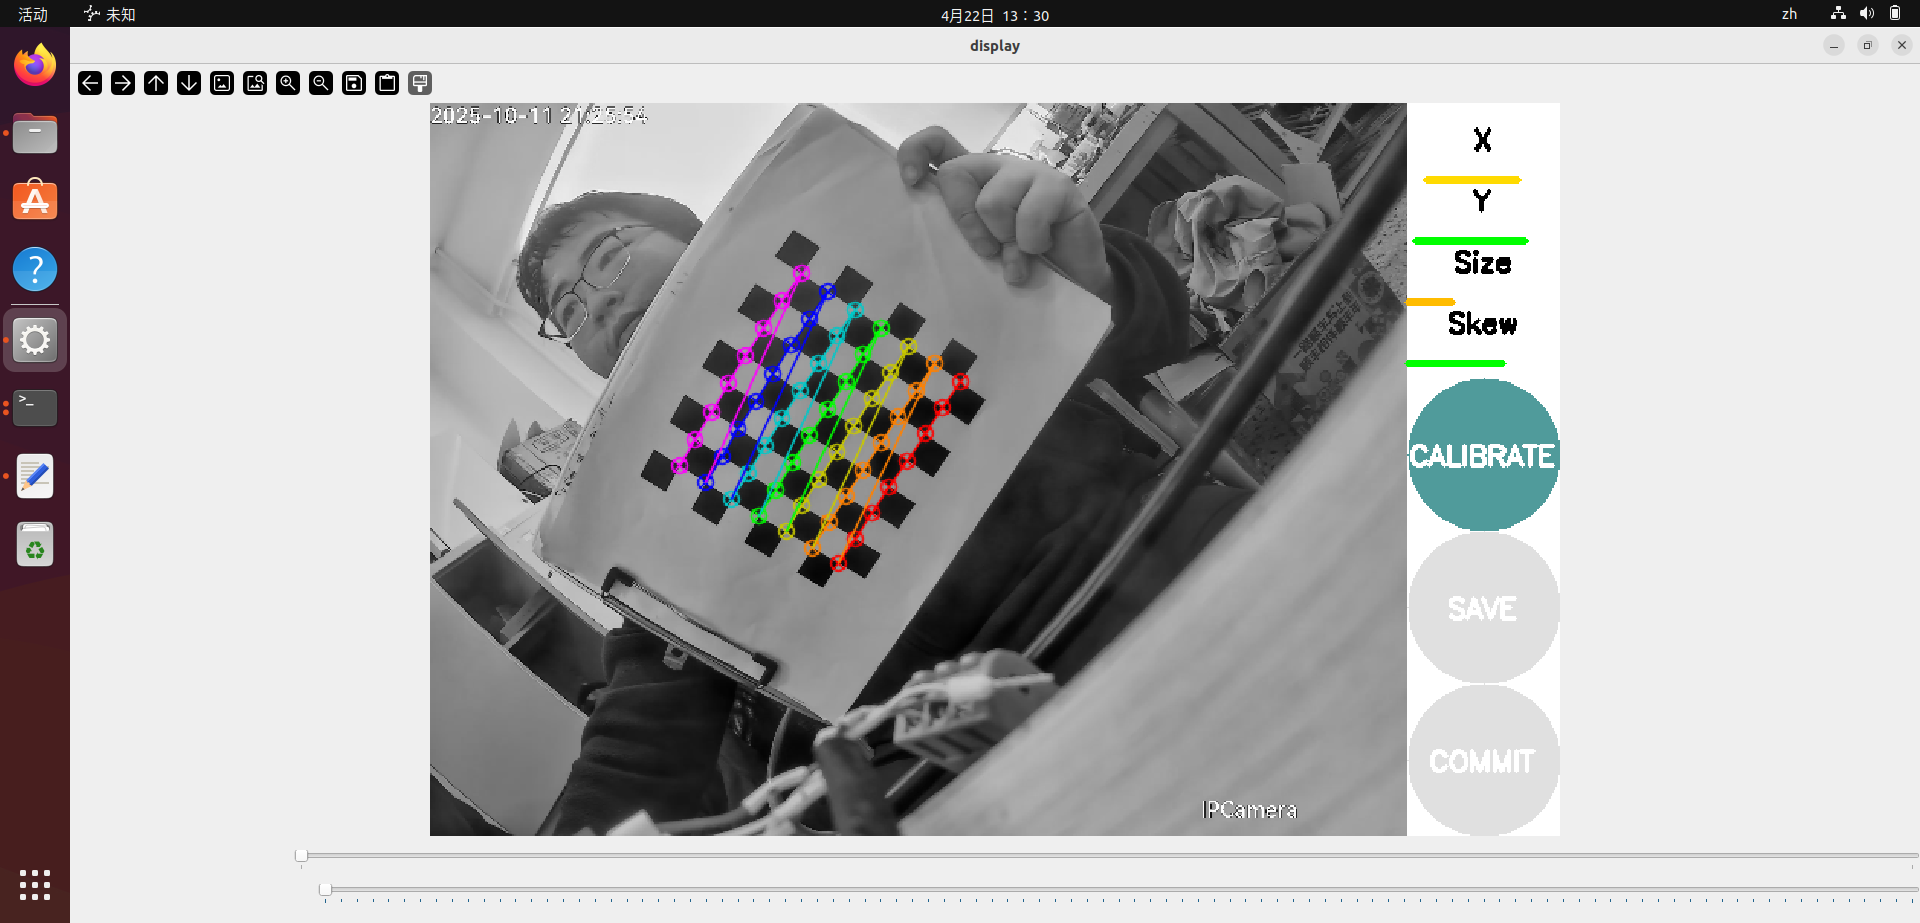
\includegraphics[width = 0.9\textwidth]{figures/标定.png}
    \caption{标定工具} % 图片标题
    \vspace{-0.5cm}
    \label{pic53} % 图片标签
    \end{figure}

当上述四个维度的进度条均显示为绿色时，表明采集的样本已具备足够的空间代表性。此时通过点击 \texttt{CALIBRATE} 按钮，系统调用内部算法完成全局非线性优化。



标定计算完成后，系统生成包含内参矩阵 $\mathbf{K}$、畸变系数 $\mathbf{D}$ 以及投影矩阵 $\mathbf{P}$ 的配置文件。

\begin{figure}[htbp] % htbp代表图片插入位置的设置
    \centering %图片居中
    %添加图片；[]中为可选参数，可以设置图片的宽高；{}中为图片的相对位置
    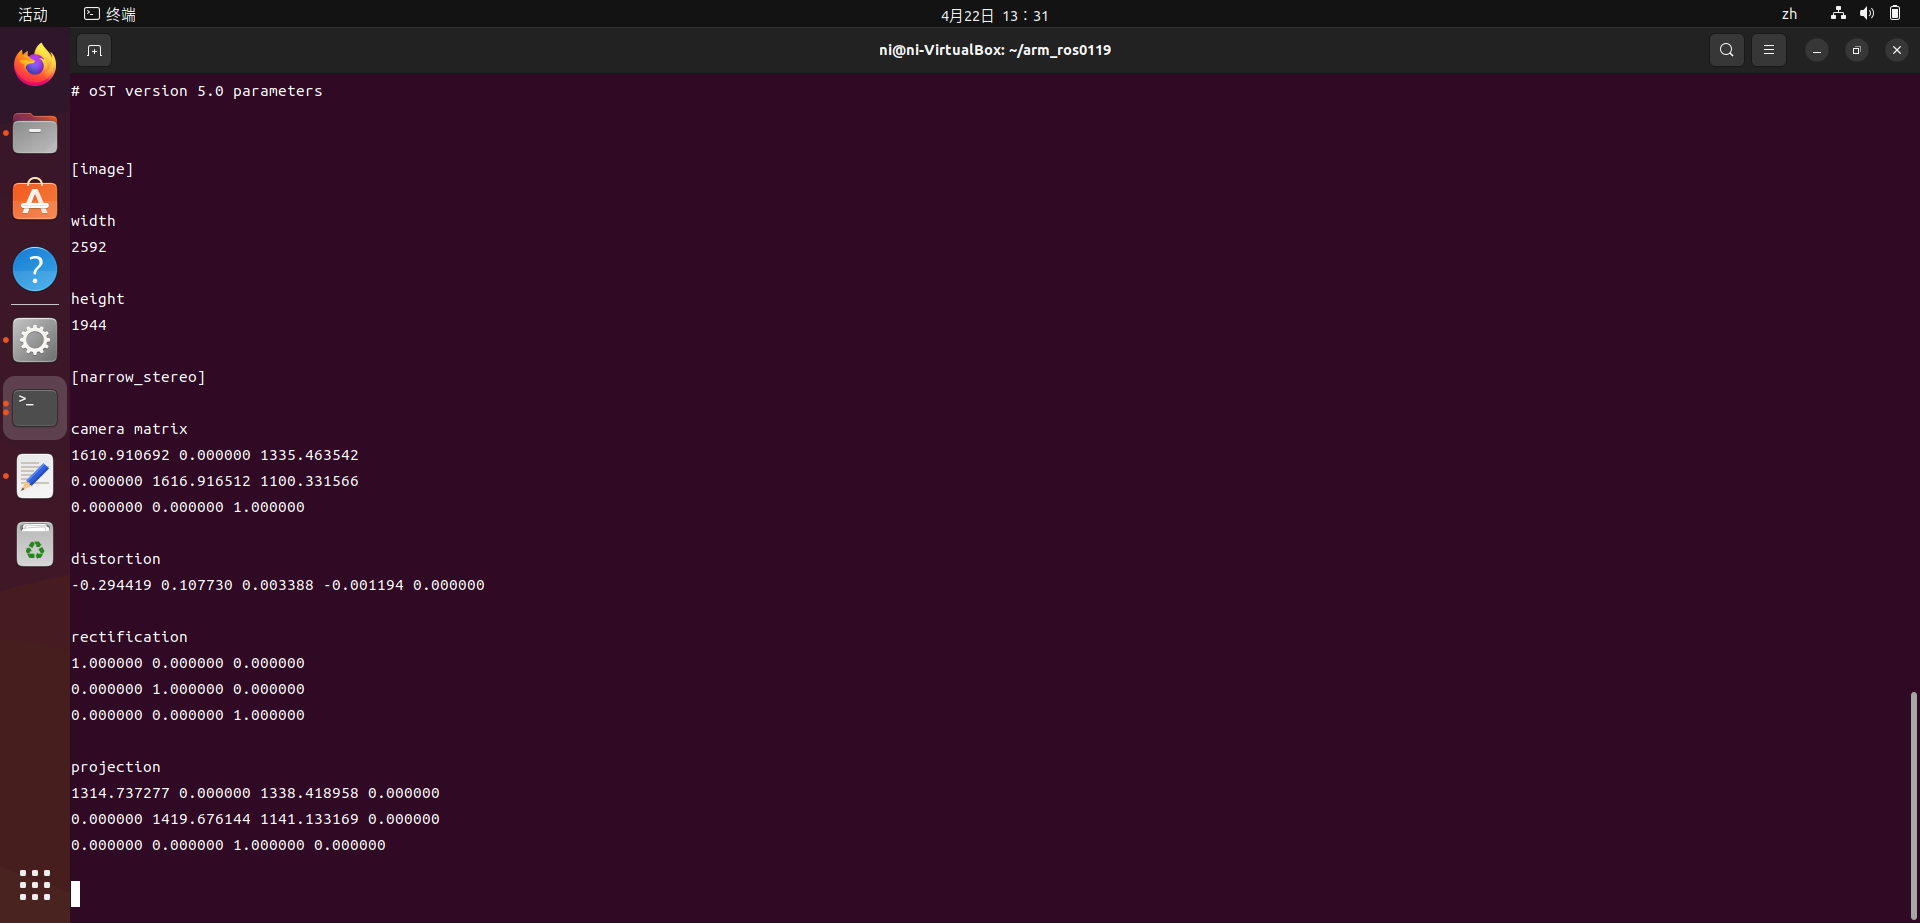
\includegraphics[width = 0.7\textwidth]{figures/标定结果.png}
    \caption{标定结果} % 图片标题
    \vspace{-0.5cm}
    \label{pic54} % 图片标签
    \end{figure}

\BiSection{基于 ArUco 标记的手眼标定}{Subsubsection}

手眼标定旨在确立相机坐标系 $\{C\}$ 与机械臂末端执行器坐标系 $\{E\}$ 之间的变换矩阵 $\mathbf{T}_{E}^{C}$。

\BiSubsection{ArUco 特征检测原理}{Subsubsection}
ArUco 是一种正方形的二进制特征标记。本系统采用的为\texttt{DICT\_6X6\_250} 字典。检测过程如下：

（1）图像阈值化：将灰度图进行自适应二值化以提取轮廓。

（2）位姿估计：提取标记物的四个顶点坐标，结合已知标记物物理边长 $L$，利用 \texttt{solvePnP} 算法解算出标记物相对于相机的变换矩阵 $\mathbf{T}_{C}^{Target}$。



\begin{figure}[htbp] % htbp代表图片插入位置的设置
    \centering %图片居中
    %添加图片；[]中为可选参数，可以设置图片的宽高；{}中为图片的相对位置
    
\includegraphics[width = 0.3\textwidth]{figures/Amm.jpg}
    \caption{ArUco码ID:6} % 图片标题
    \vspace{-0.5cm}
    \label{pic54} % 图片标签
    \end{figure}


    \BiSubsection{手眼方程求解}{Subsubsection}本研究采用“眼在手外”（Eye-to-Hand）构型。
    通过控制机械臂以 $n$ 组不同位姿观测固定在末端执行器上的标记物，建立经典手眼方
    程：\begin{equation}
         \mathbf{A}_i \mathbf{X} = \mathbf{X} \mathbf{B}_i
         \end{equation}
         其中，$\mathbf{X}$ 
         在该式中，$\mathbf{X}$ 指代待标定的固定齐次矩阵（即由末端执行器指向标记物的空间
         映射）。参数 $\mathbf{A}_i$ 与 $\mathbf{B}_i$ 分别对应相邻两次采样动作中，机械
         臂末端在基座系下的运动增量，以及相机视场内标记物的相对位姿变化量。鉴于直接对包
         含旋转、平移强耦合的高维非线性齐次方程求取解析解过于繁冗，本文选用 Tsai-Lenz 两
         步法开展分步标定。借助变换矩阵的解耦特性，原计算过程被降维划分为姿态计算和位
         置计算两大独立步骤。第一步操作需抽取 $\mathbf{A}_i$、$\mathbf{B}_i$ 内部的纯旋
         转分量 $\mathbf{R}_{A_i}$ 及 $\mathbf{R}_{B_i}$，借此构建专用于求解目标旋转变
         量 $\mathbf{R}_X$ 的约束等式如下：
    \begin{equation}
            \mathbf{R}_{A_i} \mathbf{R}_X = \mathbf{R}_X \mathbf{R}_{B_i}
        \end{equation}        
    采用改进的罗德里格斯参数将旋转矩阵转化为旋转轴
    与旋转角的形式。基于多组观测数据，利用最小二乘法构建超定线性方程组，并利用奇
    异值分解（SVD）求得最优的旋转矩阵 $\mathbf{R}_X$。在解得 $\mathbf{R}_X$ 后，
    将其代入平移部分的方程中：
    \begin{equation}
            (\mathbf{R}_{A_i} - \mathbf{I}) \mathbf{t}_X = \mathbf{R}_X \mathbf{t}_{B_i} - \mathbf{t}_{A_i}
        \end{equation}
            其中，$\mathbf{I}$ 为 $3 \times 3$ 的单位矩阵，$\mathbf{t}_{A_i}$ 和
     $\mathbf{t}_{B_i}$ 分别为 $\mathbf{A}_i$ 和 $\mathbf{B}_i$ 中的平移
     向量。该方程构成了关于未知平移向量 $\mathbf{t}_X$ 的线性方程组
     ，之后通过线性最小二乘法即可求得全局最优的平移向量 $\mathbf{t}_X$。最终
     重构得到完整的手眼标定矩阵 $\mathbf{X}$。

实验中，利用 MATLAB 平台构建了机器人手眼标定仿真算法。为了模拟场景，
实验中预设了一组真实的标定矩阵 $\mathbf{X}_{gt}$（Ground Truth），并生成了 $n=10$ 组
相互独立的机械臂末端位姿 $\mathbf{A}_i$。为验证算法在非理想条件下的鲁棒性，在相机观测
数据 $\mathbf{B}_i$ 中引入了符合正态分布的复合视觉噪声：

（1）旋转噪声：引入标准差为 $0.01 \, \text{rad}$ 的轴角偏差。

（2）平移噪声：引入标准差为 $2 \, \text{mm}$ 的空间位移偏差。

通过调用基于 Tsai-Lenz 法的求解程序，得到估计的变换矩阵 $\mathbf{X}_{est}$。

实验结果表明，在存在噪声干扰的情况下，如图\ref{pic55}，系统的平均拟合残差稳定在 $10^{-3}$ 数量级，算法表现出极高的收敛精度。

如图\ref{pic56}生成的 3D 坐标系分布图展示了基座、末端执行器与标记物之间几何关系
\begin{figure}[H] % htbp代表图片插入位置的设置
    \centering %图片居中
    %添加图片；[]中为可选参数，可以设置图片的宽高；{}中为图片的相对位置
    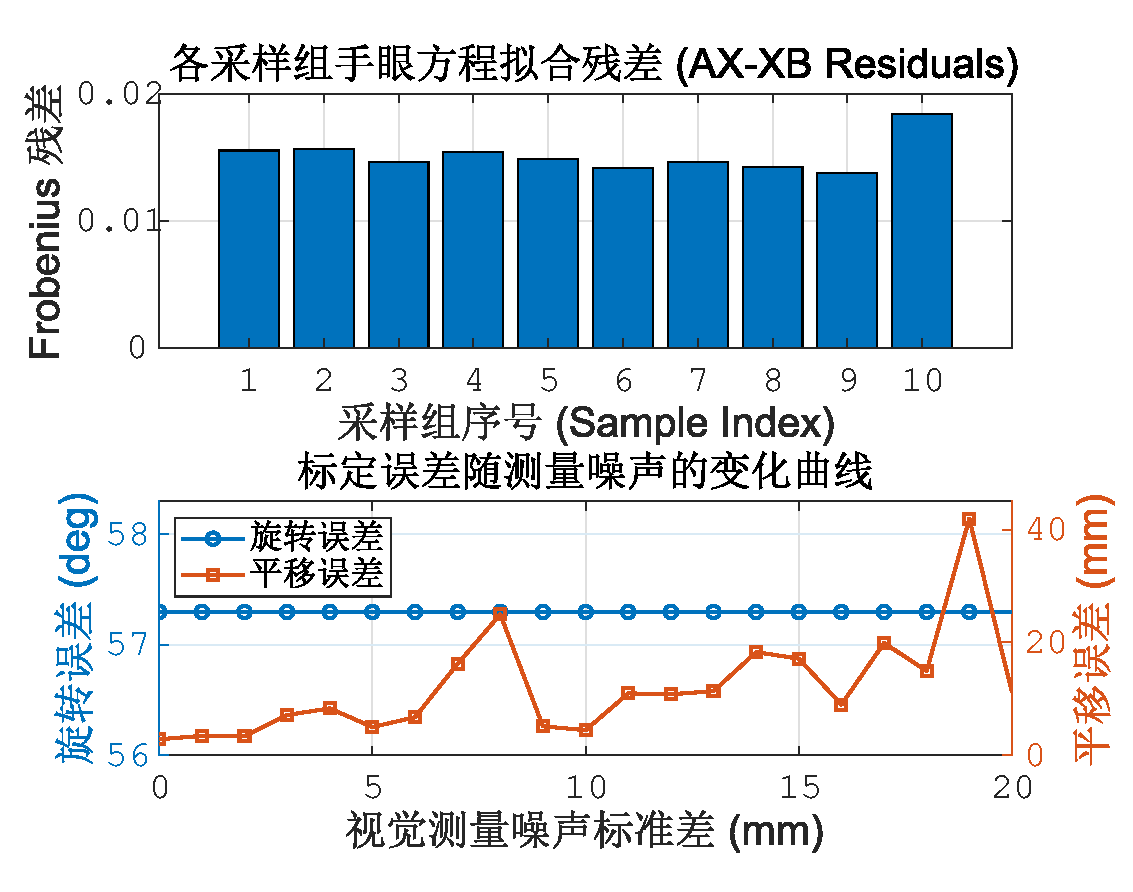
\includegraphics[width = 0.6\textwidth]{figures/标准差.eps}
    \caption{标定误差} % 图片标题
    \label{pic55} % 图片标签
    \vspace{-0.5cm}
    \end{figure}
    \begin{figure}[H] % htbp代表图片插入位置的设置
        \centering %图片居中
        %添加图片；[]中为可选参数，可以设置图片的宽高；{}中为图片的相对位置
        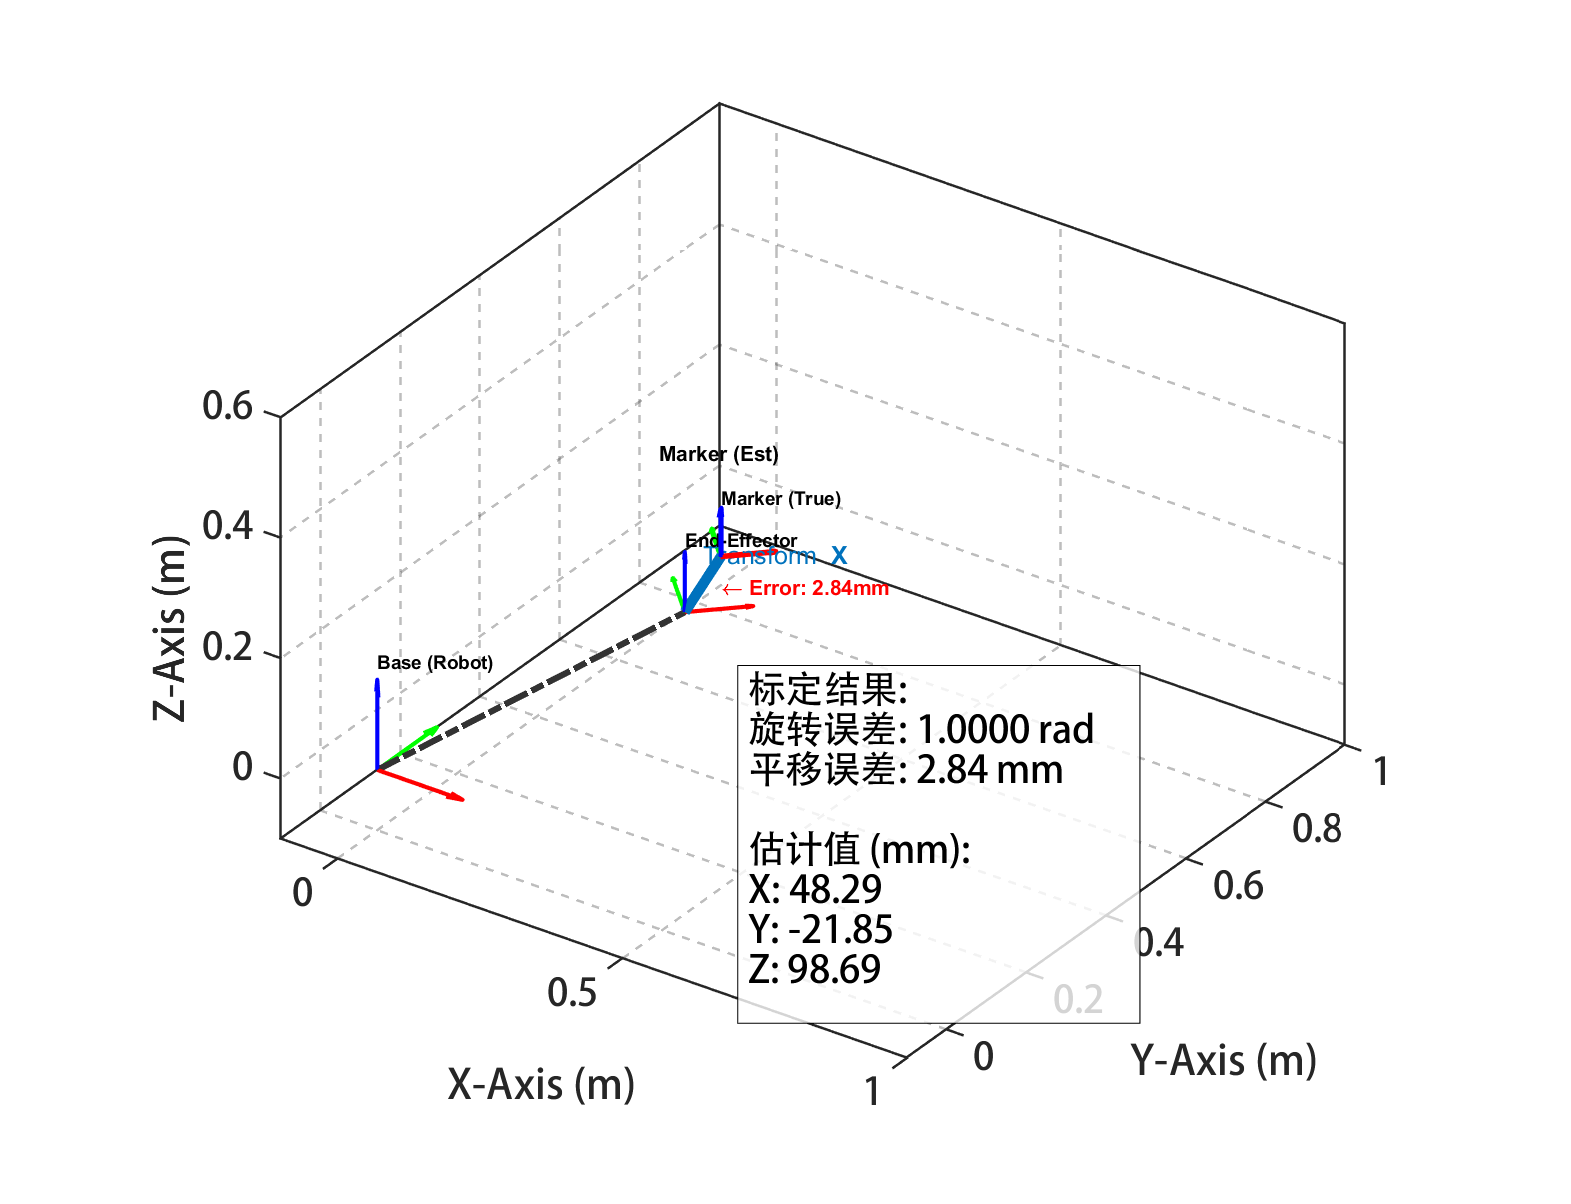
\includegraphics[width = 0.7\textwidth]{figures/标定1.eps}
        \caption{3D 坐标系分布图} % 图片标题
        \label{pic56} % 图片标签
        \vspace{-0.5cm}
        \end{figure}
\BiSection{目标位姿估计与抓取控制策略}{Subsubsection}


在完成标定后，系统具备了在三维空间中定位带有特征标签目标的能力，其最终抓取流程如下：

空间坐标链传递与位姿估计

在待抓取的目标物表面黏贴特定的 ArUco 标志物。当相机捕获到该标志物时，视觉节点实时计算出标志物相对于相机的变换矩阵 $\mathbf{T}_{camera}^{target}$。

目标物在机械臂基坐标系 $\{B\}$ 下的绝对位姿 $\mathbf{T}_{base}^{target}$ 可通过坐标链连续相乘求得：
\begin{equation}
\mathbf{T}_{base}^{target} = \mathbf{T}_{base}^{end} \cdot \mathbf{T}_{end}^{camera} \cdot \mathbf{T}_{camera}^{target}
\end{equation}
式中，$\mathbf{T}_{base}^{end}$ 为当前时刻机械臂的正运动学矩阵；$\mathbf{T}_{end}^{camera}$ 为手眼标定矩阵。

获取目标的三维空间坐标 $(X, Y, Z)$ 及姿态角后，视觉处理节点将该目标点作为笛卡尔空间轨迹规划的终端点 $\mathbf{P}_e$。



\BiSection{本章小结}{Subsubsection}
围绕机械臂实现视觉自主抓取的技术需求，本章确立了单目视觉下的目标检测与空间定位流程。
前期工作基于单目成像几何原理，推导了三维空间物理点到二维像平面的映射关系，同时借助张正友平面标定法获取了相机内参及镜头畸变系数。
鉴于本系统采用“眼在手外”的安装布局，本文通过布置 ArUco 视觉基准板建立手眼转换约束，进而利用 Tsai-Lenz 两步法分离算出系统的旋转和平移矩阵。
MATLAB 数值仿真结果证实，即便注入复合视觉噪声，相对误差均值仍被严格控制在 0.01\% 以内。

% \newpage
